%%
%% This is file 'scpe2013.tex', 
%% An invited paper with siam macros for use with LaTeX 2e, 
%% by Paul Duggan for the Society for Industrial and Applied
%% Mathematics, October 1, 1995, Version 1.0
%% 

%\documentclass[draft,a4paper]{siamltex}
\documentclass[final]{siamltex}

\usepackage{graphicx} 

\title{{ELL-i}: An inexpensive platform for fixed things}

\author{Pekka Nikander\thanks{{ELL-i} open source co-operative, Helsinki}
  \and Vaddina Kameswar Rao\thanks{Department of Information Technology, University of Turku}
  \and Petri Liuha\thanks{EIT ICT Labs, Helsinki Node}
  \and \hbox{Hannu Tenhunen}\thanks{Kungliga Tekniska H\"{o}gskolan, Stockholm}}

\begin{document}

\maketitle

\begin{abstract}
The Internet of Things (IoT) vision is enticing; each and every
``thing'' in the world is expected to be eventually connected to the
Internet, thereby becoming a part of the ``context'' within which the
applications live.  
In most of the IoT research, the focus has been in enabling
movable things to communicate, including phones, tablets, RFID tags,
watches, and jewelry, to name but a few.  In such an approach, the
things are expected to have their own batteries or receive temporary
power over short distance electro-magnetic field, and the
communications is necessarily expected to take place over radio.
This approach has also dominated the more fixed side of the
IoT research, including a large fraction on the work on stationary
sensors and actuators, focusing also there on battery-based operations
and wireless communication. 

In this paper, we introduce an alternative view to the world
of stationary things.  We argue that a large majority of the fixed or
stationary things would benefit from being permanently powered using
wireline connections, and while doing so, it becomes natural to use
the same wires also for their communication and contextual needs.
Such an approach allows the appliciances to become both part of the
the wider application context.  With this in mind,
we introduce the
ELL-i platform, a new open source initiative for provide a low-cost
flexible prototyping and production platform for extensible,
Power-over-Ethernet based smart appliances.  We describe the first
ELL-i prototyping board and briefly describe the planned technical
roadmap, a number of application concepts, and discuss its
business model. 
\end{abstract}

\begin{keywords} 
Internet of Things, Context Awareness, Direct Current (DC) power
transmission, Power over Ethernet
\end{keywords}

\pagestyle{myheadings}
\thispagestyle{plain}
\markboth{Nikander, Rao, Liuha, and Tenhunen}{{ELL-i}}

% ------------------------------------------------------------------

\section{Introduction}

Making real-life appliances intelligent and internet-connected not
only enriches the amount of environmental information available to
applications but also creates the promise of making the environment
itself a situation-aware part of the ``applications''.  As we can
easily see from the multitude of sensors that are available in today's
smartphones, once we realise the Internet of Things (IoT)
vision~\cite{Atzori20102787} of making each ``light bulb'' Internet
connected~\cite{cerf1997next}, the amount of available sensor data is
likely to multiply.  Furthermore, through making the applicances not
only sensitive but also active, the appliances may themselves become
more aware of the nearby humans, reacting and proacting in a
situation-aware manner.

Considering physical space, a key aspect of making a room, building,
or any physical space context aware is to have a sufficient number of
sensors and providing a framework for pre-prosessing the
data~\cite{Baldauf2007a}.  This is typically expected to take place
through installing a {\it sensor network} to an already existing
building or space, and routing the collected data to an aggregation
service.  In the large majority of the recent works, the sensor
network is expected to be a wireless one, to the extent that the most
widely referred referred survays carry the word ``wireless'' in their
title~\cite{akyildiz2002wireless, akkaya2005survey}.

At the same time, most of the works have implicitly ignored how the
sensors are to be powered or assume that they have a battery that will
last for their lifetime.  In general, in most of the published
research, the presented use cases and applications assume the use of
some wireless connectivity technology, although the primary ideas do
not specifically refer to specifically wireless or wired networking,
or to a any specific information and communications technology.
Looking at the situation from greenfield applications point of view,
or more widely from a sustainability perspective, assuming that the
sensors will be replaced every few, or even every tens of years, does
not look like a very rewarding alternative.

While it may well be possible to create sensor nodes that scavenge
energy from the environment and use radio or light bursts to
communicate with the environment~\cite{wang2010toward}, creating
wirelessly powered every day appliances that have some other active
function that mere sensing seems improbable.  Hence, it seems prudent
to assume that a large majority of different appliances will remain
wired, including air conditioners, blinds, coffee machines, doorbells,
electroliers, and freezers, to mention but a few.

In this paper we argue that it makes economic sense to introduce a
common open source platform for wired, communicating, intelligent
``things''.  Once established, such a platform would allow designing
and producing inexpensive appliances that are able to monitor their
(immediate) environment, participate in wider situation data
collection and perusal, and act in accordance with the users' explicit
and sometimes even implicit intentions.  In particular, we introduce
the ELL-i platform, an open source initiative that aims to provide a
low-cost prototyping and production platform for embedding wired
intelligence into buildings, appliances, and other implements.

As its first technical platform, ELL-i provides open source hardware
and software for building inexpensive embedded intelligence into
devices, allowing them to communicate and be powered with
Power-over-Ethernet (PoE)~\cite{PoE}, an established but rapidly
evolving standard for providing up to 100 Watts of electric power
through standard Ethernet cables.  The currently available ELL-i
prototyping board is compatible with the popular
Arduino~\cite{ArduinoProject} prototyping platform, with a clear path
for mass-producable miniature units that may be embedded into standard
pattress boxes within builings and most wired appliances.

The ELL-i initiative is organised a co-operative, providing an
egalitarian ownership model that anchors the property rights with the
community.  The governance model is designed to be meritocratic,
assuring that the platform will evolve in a technically sound manner.
The incentive models are designed to inspirit participation from a
wider open source developer community while still allowing mass-market
production by commercial companies.

The rest of this paper is organised as follows.  First, in
Section~\ref{sec:related} we consider related work from a relatively
wide perspective.  Then, in Section~\ref{sec:architecture} we
introduce the ELL-i platform from a technical point of view.  In
Section~\ref{sec:examples} we briefly describe some example
applications that are immediately viable with ELL-i, followed in
Section~\ref{sec:business} with a hopefully succint description of the
business model.  Section~\ref{sec:ongoing} enlists our ongoing work.
We conclude the paper in Section~\ref{sec:conclusions}, attempting to
summarise the lessons learned so far.
 
% ------------------------------------------------------------------

\section{Related work}
\label{sec:related}

\subsection{Internet of Things and Machine-to-Machine}

A first definition of Internet-of-Things (IoT) referred to identifiers
placed in objects so that they could be monitored and managed by
computers~\cite{ashton2009internet}. The idea dealt with tagging of
objects and with applications for cases like retail and logistics. It
was also related to the famous and more generic definition of the
disappearing computer by Mark Wiser~\cite{weiser1991computer} where he
described that miniaturization and ubiquity of sensors would
eventually lead to disappearing to the computational elements ``into
the fabric of everyday life''.  This has been later mentioned as
pervasive or ubiquitous computing.

One of many definitions of IoT is by Cluster of European Research
Projects (now IERC) who defined IOT as ``dynamic networked global
infrastructure with self configuring capabilities based on standard
and interoperable communication protocols where physical and virtual
things have identities, physical attributes and virtual personalities
and use intelligent interfaces, and are seamlessly integrated to the
information network''~\cite{vermesan2011internet}.

A second dimension and branch of development of IoT is the
machine-to-machine or M2M concept with further refers to linking the
plethora of digital devices (from simple microcontrolled devices to
smartphones and large industrial instrumentation). This refers more to
the communications protocols required to allow devices to communicate
with standard communications, typically wireless or even more
specifically cellular systems.  A couple of popular projects
developing the technology are the Eclipse M2M Industry Working
Group~\cite{EclipseM2M} and ITU-T Focus Group M2M~\cite{ITU-T_FG_M2M}.

In general, IoT devices can be used to design products and services
which can be enhanced by
data connectivity and can provide intelligent feedback back to the user.
Proliferation of cheap and versatile sensors, actuators, computing, storage and
networking solutions augmented by the desire to connect people with their
devices in a more meaningful way have contributed significantly to the IOT
research. IMS research predicts that there will be 30 billion devices which will
be connected to the Internet by 2020~\cite{ABIresearch}. Most of the IOT
research has been used to serve diverse domains of wireless and RFID based
applications with built-in powering solutions. In this work we focus on an
alternative way for providing both the communication and powering solutions to
fixed and immovable devices, which would anyhow be powered by wirelines, using
Power over Ethernet (PoE) standard.

\subsection{Internet of Things applications}

Internet-of-Things applications include a variety of applications
ranging from vehicle telematics, tracking and tracing of objects to
applications applying wireless sensor networks and machine-to-machine
(M2M) systems. Typical applications are in military use cases (like
intelligence, surveillance), environmental use cases (e.g. monitoring
conditions that affect farming and animal husbandry, or monitoring
macro-scale phenomena in soil, forest, marine or atmospheric
contexts), health applications (remote monitoring of patients, tracing
of care personnel or equipment), home applications, or other
commercial applications like interactive smart spaces in office or
other working environments.

The use cases include applications with large area networks and high
mobility but also no-mobility use cases. Wu~et.~al. discusse the
requirements for future applications from the M2M
perspective~\cite{wu2011m2m}. While many of them assume wireless
connectivity, a good part of them are in fact for fixed things, like
in home management, industrial automation and metering, sensors, and
lighting. More generically IoT use cases with no mobility exits in
smart homes or smart buildings and smart cities e.g. for the purpose
of reducing the consumption of resources associated to buildings
(electricity, water) or improving the satisfaction level of humans
populating them~\cite{miorandi2012internet}.

\subsection{Power management and security in IoT and M2M research}

In this work, IOT devices have been classified by the amount of power required
for their efficient operation. Some IOT devices use batteries, some scavenge
energy from radio waves (RFID and NFC), while others are powered by seperate
power supply from the mains (like PoE).  The main roles of IOT devices include
sensing, collecting, processing, transmitting, collaborating and communicating.
All of these roles require power to accomplish. Smart and tiny embedded systems
have sensors, actuators, CPU, memory and a low-power communication
device~\cite{lopez2012adding}. Usually, these can be powered by a battery. On
the other hand, Wireless Sensor Networks (WSN's) which is a popular research
area uses energy efficient battery powered wireless devices for transmitting
sensor data~\cite{akyildiz2002wireless}.

Security:
For the case of mobile devices, as the complexity of the encryption algorithm
increases, their battery consumption increases as well. It has been shown that
among symmetric encryptions used in security protocols, the AES128 algorithm
increases the battery consumption and the processing time by 75\% and 65\%
respectively when compared to "no encrption" results~\cite{hamad2009energy}.
Furthermore, increasing the key size for the encryption also increases the
battery consumption and processing time. That is, increasing the keysize from
128 bits to 192 bits results in 8\% increase in power and time consumption and
16\% increase when the key size is increased to 256
bits~\cite{hamad2009energy}.

\subsection{Digital power management in general}

The industry has been challenged to provide digital power-management solutions
which can communicate with various connected systems that inhabit our world.
Digital power-management protocols like the PMBus could not be moved to the
board level and provide real value to the designer before the introduction of
intermediate-bus architecture~\cite{FutureIOT}. It would have been difficult to
foresee the interdevice communications for both power and data without the
advances in mixed-bus connector architectures, such as USB and PoE (power over
ethenet)~\cite{FutureIOT}. 

A Power-over-Ethernet system can communicate with its power source
bidirectionally for both power and intelligence. This can provide new and
innovative ways to develop power management methodologies inorder to raise the
overall power efficiency of the system.

%
% Condense the following three chapters into a message about power
% requiremnts here
%

The smallest RFID chip manufactured by Hitachi is at 0.05mm $\times$ 0.05mm
$\times$ 0.005mm. It can respond to 2.45GHz microwave from a scanner by
reflecting back a unique 128-bit ID number. It can be read from 30cm away and
requires no batteries or power supply~\cite{hornyak2008rfid}.

It would be a daunting logistical challenge to experiment with thousands of
battery-power nodes which has been limiting the development of this
field~\cite{gluhak2011survey}. Also, indoor installation and usage of nodes
provides easier access to power and cabling~\cite{gluhak2011survey}. Although,
nodes maybe cheap, their deployment and maintainance is an expensive
proposition.

It is possible to use the energy harvested from the environment to power
nanosystems which have the capabilities to sense, control, communicate and
actuate/respond~\cite{wang2010toward}. For independent, sustainable,
maintainance-free operations of implantable biosensors, remote and mobile
environmental sensors, nanorobotics, micro electromechanical systems, and even
portable/wearable personal electronics require power on the scale of
microwatts~\cite{wang2010toward}. Wang~\cite{wang2010toward} has invented a
nanogenerator which can convert random energy (the mechanical energy which is
available in our environment and has wide spectrum of frequencies and
time-dependent amplitudes is defined as random energy. It can come from various
sources like irregular vibrations, light airflow, ambient noise and other human
activity). The nanogenerator converts random energy into electrical energy using
piezoelectric zinc oxide nanowire
arrays~\cite{wang2006piezoelectric}\cite{yang2009converting}. A gentle straining
on the array of nanowires can output 1.2-3V, which can drive a self-powered pH
and UV nanosensor~\cite{xu2010self}, liquid crystal display and light emitting
diode~\cite{xu2010piezoelectric}\cite{zhu2010flexible}. Although the power that
is generated by the nanogenerator may not be sufficient for continuous operation
of a nanodevice, it is sufficient enough to drive the device for a few seconds,
when the charge being generated is accumulated over a period of
time~\cite{wang2010toward}. This would have practical uses when the device has
active and standby modes, such a glucose sensors, blood pressure sensors and
bluetooth transmitters (driving power \~5mW; data trasmission rate \~500kbits/s;
power consumption of 10 nW/bit) which are required to be in active mode
periodically~\cite{wang2010toward}.

\subsection{Single-wire powering and communication solutions}

\begin{itemize}
  \item PoE
    \begin{itemize}
    \item 802.3af, 802.3at, non-standard solutions to up to 65W or so
    \end{itemize}
  \item Ethernet-over-Powerline
  \item Others
\end{itemize}
 
\subsection{Open source embedded platforms}

\begin{itemize}
  \item any other similar PoE platforms: Arduino PoE, etc
    \begin{itemize}
    \item technical difference from these
    \item governance difference from these
    \end{itemize}
\end{itemize}

Today, there are a few tens of slightly different open source embedded
platforms.  The Raspberry Pi~\cite{RasPi} forms a category of its own,
offering an unbeatable price point in the embedded Linux category.  In
the lower category, the Arduino~\cite{ArduinoProject,hribernik2011co}
project has gained the largest user community, with half a dozen
different official boards and a number of derivatives~\cite{XXX}.

XXX

The Arduino project is a somewhat loose collaboration led by a number of
people that developed the original Arduino design.  They have decided
to open source all of the software and hardware but to keep the
Arduino and associated graphics as trademark.  At the moment there are
three companies that are authorized by the project leaders to produce
official Arduino boards~\cite{ArduinoPolicy}.  The financial
arrangements between the project leaders and the authorised
manufacturers are not known.

The Raspberry Pi is produced by the Raspberry Pi Foundation, which is
a UK registered charity founded in May 2009 in Caldecote,
Cambridgeshire, UK, supported by the University of Cambridge Computer
Laboratory and Broadcom~\cite{RaspiFoundationWikipedia}.  For its
first three years of operation, the foundation income was annually
less than \textsterling 10.000.  The foundation income and spendings for 2012
were not registered at the UK Charity Commission at this writing.

There are other Arduino and Raspberry Pi based PoE
solutions~\cite{ArduinoEthernetPOE} \cite{ArduinoEthernetShieldPOE}
\cite{POEthernetShield} \cite{etherduino} \cite{xtronix} currently available in
the market. Some of them are complete PoE solutions while others are shields
that can be plugged into an Arduino. The Arduino Ethernet with
PoE~\cite{ArduinoEthernetPOE} is an Arduino development board with the built in
Wiznet Ethernet interface. Although the board can be powered over the Ethernet
connection, the developers have removed the USB-serial driver and hence it will
need an FTDI breakout to upload Arduino sketches. The Arduino Ethernet Shield
with the PoE Module~\cite{ArduinoEthernetShieldPOE} allows an Arduino board to
connect to the internet. It is based on Wiznet W5100 ethernet chip which
provides a network IP stack capable of both TCP and UDP. The PoEthernet
Shield~\cite{POEthernetShield} gives access to the Internet via the Ethernet
library and also allows the Arduino based projects to power itself from the
Ethernet line. The Raspberry Pi Power Over Ethernet (PoE) Adapter~\cite{xtronix}
manufactured by Xtronix Ltd, is designed to be plugged directly on to a
Raspberry Pi and power it with +5 Volts at up to 1.0 Amps output. All of these
solutions are either expensive and/or bulky to reside in a pattress box.

The long term vision for ELL-i differs significantly from those of other PoE
solutions that are described here. ELL-i is a multi-voltage domain design and
both the PoE 48V or the DC-to-DC converters can be used. ELL-i is aiming to be
an inexpensive low-cost PoE device which will come with integrated cloud based
services pre-loaded out of the box. When it is ready, the ELL-i board will be
around 45 $\times$ 45 $mm^2$ and can easily fit into DIN pattress boxes. 


% ------------------------------------------------------------------

\section{ELL-i platform architecture}
\label{sec:architecture}

In this section, we describe the ELL-i technical architecture in
sufficient detail to ground the discussion that follows\footnote{For further
details, please refer to the open source design files at
\hbox{\tt http://www.github.com/ELL-i}.}.
First, we describe the overall technical architecture in a
bottom-up-fashion, including hardware, firmware, and the forthcoming
could components.  After that, we introduce the current
implementation and discuss the plans for the next hardware implementation.  We
conclude the section with a brief discussion of the design choices
made so far.

\subsection{Overall technical architecture}

The ELL-i platform consists of a hardware architecture, a runtime
(firmware), cloud-based components, and support for a set of
programming environments.  The basic architecture is depicted in
\ref{fig:arch}.

\begin{figure}
\centering
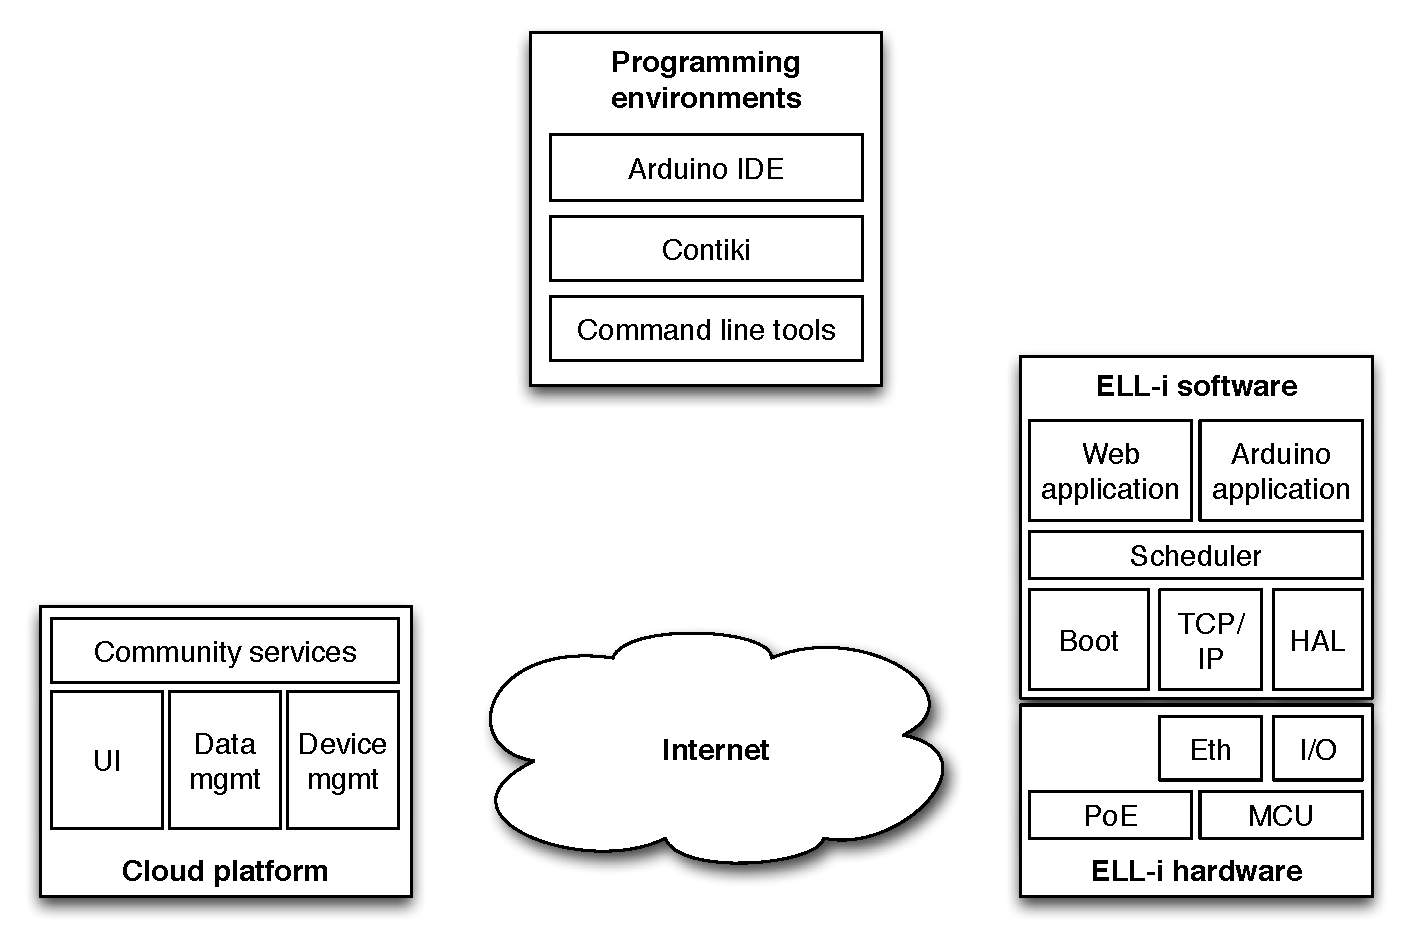
\includegraphics[scale=.4]{figure-arch.eps}
\caption{ELL-i platform architecture}
\label{fig:arch}
\end{figure}

The hardware architecture is based on combining power and
communications on a single cable, making both of them available to
applications.  In practise, the current implementation is based on the
IEEE 802.3at Power-over-Ethernet standard, which is an economic
solution when the power consumption is roughly in the 1--100 Watts
range.  In the long run, we expect to expand the power range to both
smaller and higher power levels; for example, there are no technical
reasons why Power-over-Ethernet could not be applied to thicker wires
and higher currents.

The main goal of the runtime and the cloud components is make it easy
to provide connectivity for the appliances.  Hence, the goal of the
runtime is to package TCP/IP based protocols, such as HTTP~\cite{HTTP}
and CoAP~\cite{CoAP} in an easy-to-use way.  As it is undesirable to
perform packet processing in an interrupt context and as many of the
protocols depend on timeouts, abstracting the protocol processing away
from the runtime API requires some kind of threading, either in the
``scouts honour'' style (as in e.g. Contiki~\cite{Contiki-scheduler})
or in a proper pre-emptive manner.  At this writing it is still an
open question which variant we will primarily support.

As ELL-i is positioned as an easy-to-start platform, the main goal in
the programming environment area is to make it easy to start with the
ELL-i platform.  Hence, we have focused on providing an Arduino IDE
extension that allows Arduino skills to be readily applied on ELL-i.
However, we also realise that the default Arduino runtime is geared
for hobbyists.  Therefore we will also support XCode and Eclipse, most
probably by adopting the existing Arduino plugins.

\subsubsection{Hardware}

In practice, the platform hardware consists of an MCU, an Ethernet
communications module, a power supply module, and an I/O subsystem
that connects the system to the real world.  The MCU provides the
smarts, including a computational core, non-volatile (flash) and
volatile (RAM) memory, and peripherals for connecting with the
communications, power, and I/O subsystems.  It executes a program
stored into its flash, converting commands received over the Internet
into changes into its I/O state and vice versa.  The MCU program is
primarily responsible for implementing the TCP/IP protocols.  In a
typical case, it takes also (partial) responsibility on controlling
the DC/DC power supplies, thereby reducing the overall cost of the
system.

The Ethernet communications module implements the IEEE 802.3~\cite{802.3}
communications standard, sharing the same cable with the PoE-based
powering of the device.  It consists of three components: the
isolation magnetics, the physical interface (PHY) and the media access
control interface (MAC).  The firmware takes care of the actual packet
processing.

The power supply module consists of an Power-over-Ethernet signalling
module and a DC/DC power supply module.  The former implements the
IEEE 802.3af~\cite{802.3af} or 802.3at~\cite{802.3at}
Power-over-Ethernet standard, including the physical-layer signalling
that consists of an initial resistive-load based detection phase, a
current-sink based classification phase, an optional second
classification mode added in 802.3at, and an operating-voltage rampup
phase~\cite{802.3at}.  We will implemente the Ethernet Layer 2
based advanced power management~\cite{802.3at} later.

The DC/DC power supply is responsible for converting the incoming
Power-over-Ethernet 48V voltage into the 5V and/or 3.3V needed by the
MCU and other digital electronics.  In a specific ELL-i application,
there may be an additional power supply producing ``bulk'' power for
the ``real world'' components, such as a constant-current PSU for a
high power LED light, a circuit generating suitable current pulses for
a solenoid, or a precicely controlled PSU generating modulated
currents for a direct-current driven electric motor.  In most real
world applications there is a difference between the power
requirements of the digital electronics, which typically require
constant voltage but variable current, and that of the real-world
actuators, which typically require controlled current but are
relatively insensitive to the actual voltage.

Finally, the I/O subsystem adjust the electical signals generated by
the sensors and required by the actuators with the levels created and
tolerated by the MCU.  In a typical case, the I/O subsystem consists
of operational amplifiers acting in amplifier and/or level shifter
role.  In many cases also optoisolators or other isolators are needed.

In a typical application, the I/O subsystem needs application-specific
design or adjustments.  Perhaps more importantly, when the ELL-i
platform is used for driving real world actuators, in most cases there
is also a need for an application-specific DC/DC converter.  ELL-i
attempts to make designing and building both of these customisations
easier than what the state-of-the-art has been so far.

\subsubsection{Runtime}
\label{sssec:runtime}

The runtime system forms the bases of any firmware running on the
ELL-i platform.  In practise, it consists of a software library that
is linked into any specific firmware build by an application
developer.  The runtime provides a number of APIs and services that make
application development easier than building everything from scratch.

In ELL-i, the main goals of the runtime are to provide an
easy-to-start but still powerful programming environment for both
novices and professionals, and to offer facilities for communicating
with the cloud components in the Internet.  To achieve that, the ELL-i
runtime consists of a boot module, a hardware abstraction layer (HAL),
a tiny scheduler providing concurrency, an Internet-communications
module, an optional built-in Webserver, and a set of APIs providing
programmatic access to all of these.  The runtime architecture is
illustrated in Figure~\ref{fig:software}.

\begin{figure}
\centering
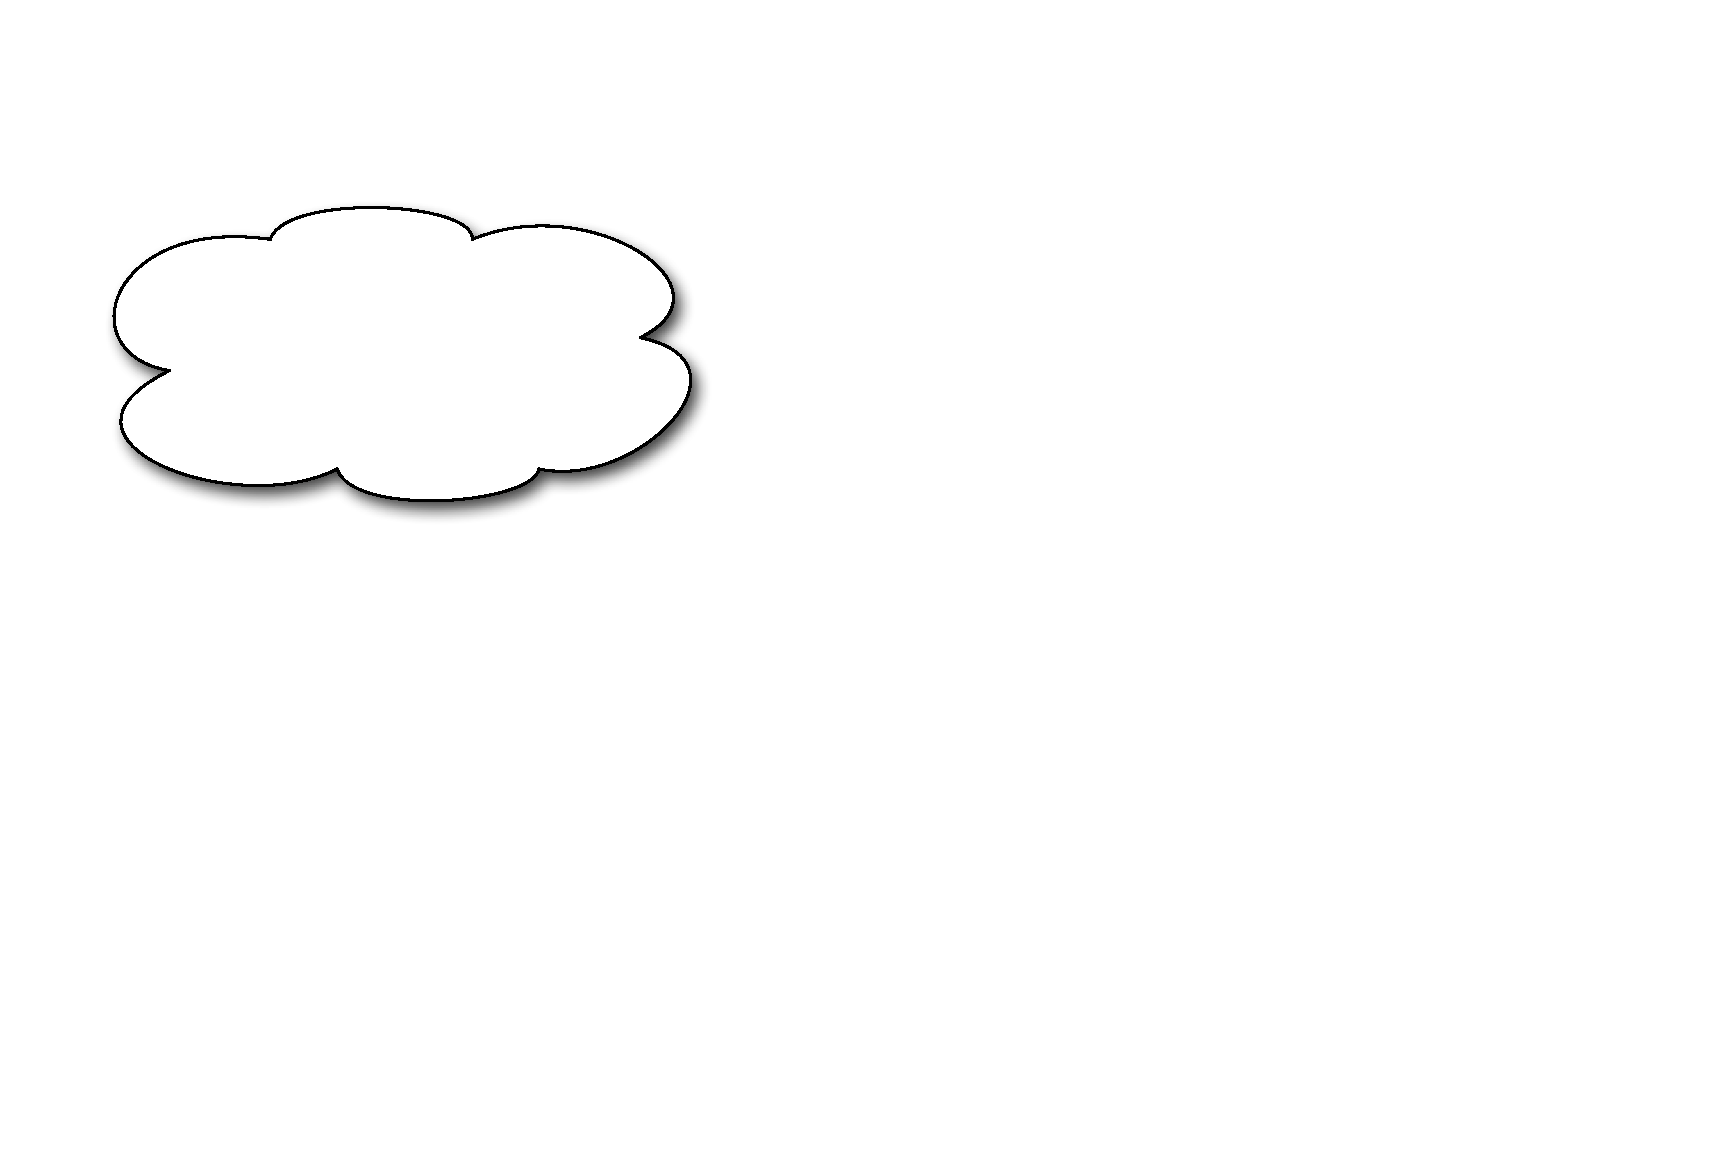
\includegraphics[scale=.4]{figure-software.eps}
\caption{ELL-i runtime architecture}
\label{fig:software}
\end{figure}

The set of APIs may be devided into five groups, corresponding to the
booting, HAL, scheduler, Internet, and Web-services.  In the current
implementation, the boot and HAL APIs provide an Arduino-compatible
programming environment, allowing programmers to initialise the
hardware using the familiar \hbox{\tt setup()} function and to run a
main loop within the \hbox{\tt loop()} function.  Both of these are
called by a \hbox{\tt main()} function, allowing more advanced
programmers to override the Arduino approach.  The familiar Arduino
HAL APIs are supported, such as accessing GPIOs and serial lines.

While the original Arduino runtime does not provide any concurrency,
thereby causing e.g. busy loops to stall the whole MCU, in the ELL-i
runtime there is a small scheduler running ``under'' the Arduino
APIs.  Using the scheduler, the Internet and Web-server modules are
implemented so that they always run concurrently with any Arduino
sketch.  More advanced programmers that override the \hbox{\tt main()}
function must include a call to initialise the scheduler.

The scheduler API provides services for starting and stopping concurrent
threads and adjusting the scheduling algorithms.  By default threading
is fully pre-emptive, allowing the TCP/IP stack to work on a higher
priority than any Arduino sketch.  Any I/O modules requiring precise
timing need to run on their own threads, or in their interrupt
context, in order to preempt packet processing.  Dynamic memory
management is not supported and is strongly discouraged; any threads
need to have their stacks to be allocated at compile time.

The Internet API provides basic services for operating TCP, UDP and
CoAP\cite{CoAP} sockets.  The TCP/IP stack is based on
uIP~\cite{uIP}, with the
uIP API working as such.  We plan to support Contiki~\cite{Contiki}
style protothreads~\cite{protothreads}, thereby making it easier to
support existing uIP-based protocol stacks and applications.

The optional built-in Web-server allows the ELL-i platform to provide
AJAX-style Webservices towards the local network.  For security
reasons, the TCP packet lifetime is limited to one hop, thereby making
the webservice unreable from the Internet even in the case the node
has a public IP address and full internet connectivity.

The runtime library has been carefully built in a way that allows the
linker to leave out any modules that are not used by a particular
application.  However, whenever the default \hbox{\tt main()} function
is used, the runtime includes the UDP/IP stack, the CoAP protocol, and
a basic service module that registers the node with the cloud
components and by default sends sensor data to the cloud.

\subsubsection{Cloud components}

In addition to the software components running on the ELL-i hardware,
the ELL-i platform contains also cloud components, running on a
compatible cloud runtime, such as AWS~{AWS} or AppScale~{AppScale}.
The cloud components provide interaction, update and community
services to the ELL-i boards, and they are enabled by default in each
ELL-i development board.

In the default configuration, a newly installed ELL-i development
board attempts to contact its counterpart component at the cloud
side, making the cloud-side component aware that the board is running
and has Internet connectivity.  At the same time, the user may direct
their browser to a board-specific URL and view the board status.  The
board may also peridically send sensor information to the cloud, such
as a reading from the MCU-internal temperature sensor.  This data is
then visualised to the user.

Another cloud-based service is the ability to remotely upgrade the
firmware on ELL-i boards.  If the remote upgrade is enabled, the
firmware contains a tiny CoAP-based communications module that is able
to download new firmware page-by-page to the RAM, and flash it.  By
default, each page must be protected with a symmetric cryptographic
key, shared between the board-specific cloud component and the board
itself.  If the remote upgrade fails and the board no longer boots, it
still remains possible to completely reflash the board using a serial
line and a separate programming board.

We are also contemplating of including community services to the cloud
side, such as allowing the developers to see (but not modify) some of
the cloud-side data of other developers' devices.

\subsubsection{Programming environments}

The ELL-i platform is designed to support multiple programming
environments, including the Arduino IDE, Eclipse, XCode, and for the
old timers, plain \hbox{\tt emacs} and \hbox{\tt make}.  At this
writing only the Arduino IDE is formally supported, even though some
of the early adopters do use command-line tools.  The aim is to make
it {\it easy} to move from the Arduino IDE to the more advanced
programming environments, with clear instructions how to convert
Arduino sketches into proper C++ source files.  This also requires
clear explanations of what is happening under the hood in the runtime.

On the compiler side, at the moment we are still using the very GCC
version provided by the default Arduino IDE.  However, our plan is to
move to LLVM~\cite{LLVM} as soon as possible, and to enable global
link-time optimisation.  This together with well-written static
initialisation of global C++ objects, such as the Arduino \hbox{\tt
  Serial}, allows the compiler in many cases to optimise away not only
virtual function calls but use constant propagation down to the level
where the Arduino syntactic sugar may be optimised completely way,
providing the same level of efficiency as would normally be
achieveable through bare-metal access while still working with
high-level C++ abstractions.  We are also considering whether it would
be possible to pre-run the Arduino \hbox{\tt setup()} function and
some of the preceeding setup machinery during the compilation
time\cite{Rinta-aho_et_al}, providing boot-time optimisations.

\subsection{Current implementation}

At this writing in September 2013, the currently available
implementation consists of the first prototyping board, an initial
runtime, and support for the Arduino IDE.  Work on the cloud-side
components will be started later.
The goal of the first prototyping board was to create
Arduino-compatible hardware and software that would support a more
powerful
MCU than the present basic Arduinoes do and to allow custom DC/DC
power supply design.  This goal has been reached.  With the first
prototyping board, prospecting developers can utilise the existing
Arduino examples, learning material, and shields, to a large extent.

\subsubsection{First prototyping board}

The first ELL-i prototyping board was designed during spring 2013, and
the first batch of 50 boards arrived in the end of May.  These initial
boards have an STM32F051\cite{STM32F051} ARM Cortex-M0
microcontroller, Microchip ENC28J60\cite{ENC28J60} Ethernet chip,
Linear LTC4267 PoE controller with build-in flyback SMPS controller,
and Arduino-compatible headers.  We also have a 3D printed case for
the prototyping board, with enough of space for a few Arduino shields.

The STM32F051 MCU was selected partially because it was already
familiar to us, partially because it represents a relatively new
Cortex-M MCU at an attractive price point compared to the included
peripherals.  We also appreciate the fact that the STM32F050 and
STM32F060 MCUs are potentially even cheaper choices when considering
mass production.  The STM32F051 is also available at an 64-leg LQFP
package which is essentially pin compatible with its bigger brothers,
up to STM32F4 Cortex-M4 series.

The old and tried ENC28J60 was selected for its low price and good
software support, even though it has its known quirks.  As a chip that
contains both the Ethernet PHY and MAC layers it provides a unique
combination, saving both silicon and pins at the MCU end, thereby
leading to an optimised overall pricepoint.

At the PoE side, Linear LTC4267 was chosen relatively blindly, as we
had little understanding of the PoE PD chip choices when we started.
Its evaluation kit worked nicely and it was easy to copy the
schematics for our purposes.  At it works, it appeared to be a good
choice for the initial design.  For the next round, we need to
evaluate more alternatives.

For Arduino-compatibility, we designed the LTC4267-based flyback DC/DC
converter to produce 5V, using a standard linear regulator to produce
3.3V out of the regulated 5V supply.  That allows us to replicate
Arduino Due and Arduino Mega I/O pins with some accuracy.  We left out
the ``east'' end headers, though, as there are clearly fewer I/O pins
available in the 64-pins package than is available in either Due or
Mega.  At the moment the I/O pins have been assigned so that there is
a separate timer/counter channel available for all of the digital I/O
pins, an ADC channel for all of the analog pins, and the DAC on the
STM32F051 is connected to the Due DAC0 line.  At the moment, the Due
DAC1 line is connected directly to the STM32F051 PA11 GPIO line;
however, we are considering adding there a low pass filter to allow
the attach PWM counter/timer to be used to generate analogue signals.

\begin{figure}
\centering
\includegraphics[scale=.4]{figure-casedesign.eps}
\caption{ELL-i case design}
\label{fig:casedesign}
\end{figure}

The current case design is depicted in Figure~\ref{fig:casedesign} and
a corresponding prototype in Figure~\ref{fig:case}.  The prototype has
been printed with the MakerBot II~\cite{MakerBotII} 3D printer.

\begin{figure}
\centering
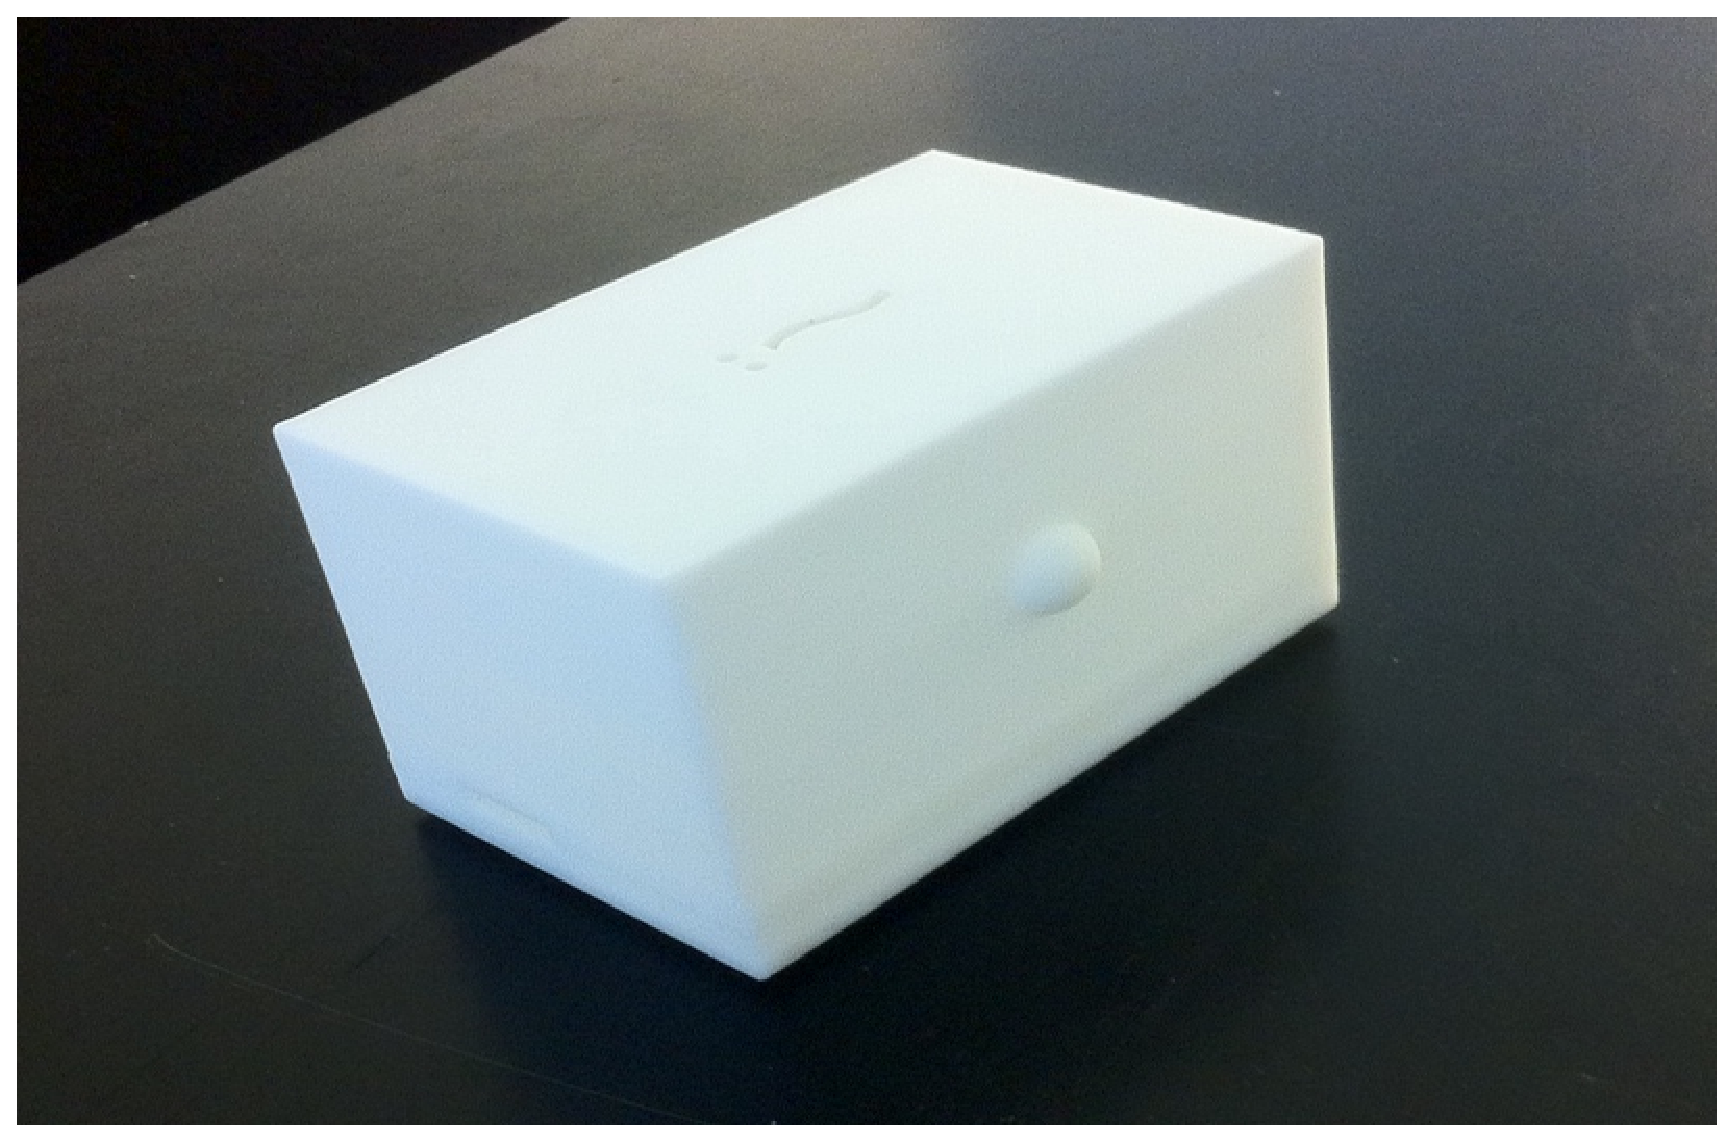
\includegraphics[scale=.4]{figure-case.eps}
\caption{ELL-i 3D-printed prototype case}
\label{fig:case}
\end{figure}


\subsubsection{Runtime and Arduino IDE support}

As the first programming environment, we have been focusing on
supporting the Arduino IDE.  Starting with the Arduino IDE 1.5
extension mechanism~\cite{ArduinoIDEextension}, we have developed our
own Arduino-compatible runtime that compiles about over 90\% of the
sketches provided with the Arduino IDE.  However, while most of the
APIs are supported at the syntax level, there is still quite some
underlying code missing so that only some 40-50\% of the API
functionality is supported.  The existing functionality is enough for
many of the basic sketches, though, thereby helping people to get
started with ELL-i.

At the moment we are busy implementing the first version of our
scheduling system, after which we will be able to provide TCP/IP
support with uIP.  XXX UPDATE!

\subsection{Ongoing efforts}

When designing the first prototyping board, our goal was to learn how
to build Arduino-compatible boards and how to provide an Arduino
compatible IDE with that.  We have clearly reached that goal.  With
the next board, we want to go further.  A major goal of this present
design round is to allow people to easily extend their designs from
the Arduino world into real-world embedded applications, allowing
real-life creation of intelligent and connected fixed appliances.

\subsubsection{Hardware design in progress}

While the first prototyping board was produced as a single PCB in the
Arduino Due/Mega form factor, the next hardware revision is based on
the idea of using two separate boards in a sandwich fashion.  In
addition to that, we plan to add support for 12--60V DC operations allowing
the boards to be used independently from Power-over-Ethernet, for
multiple MCU versions ranging from STM32F050 to STM32F407, for
optional real time clock, operational amplifiers, level shifter, and
driver FETs.  Finally, in addition to the current plastic case our
plans include a sturdy metal case.

{\bf Two-board design.}
There are two reasons for having two boards instead of one.  Firstly,
we learned from the first board that the standard RJ11 Ethernet
connectors and the typical flyback transformers are so high that they
do not fit in to a board with standard-height 100mil
headers\footnote{It the PCB industry, it is a standard practise to
  space the pins on older component packages and larger connectors at
  100mil or 0.1 inch spacing (2.56 mm).  The female connectors in the Arduino
  boards do this.  The standard 100mil female header height is
  typically around 8 mm, while even the lowest RJ45 sockets
  are around 14 mm.  This makes it challenging to produce
  Arduino-compatible boards with standard-height headers.}.
Having two boards stacked in a sandwich fashion allows us to place the
high components on the lower PCB and the Arduino-compatible 100 mil
headers on the upper PCB.  In this way we can use standard-height
connectors; see Figure~\ref{fig:stacking}.

\begin{figure}
\centering
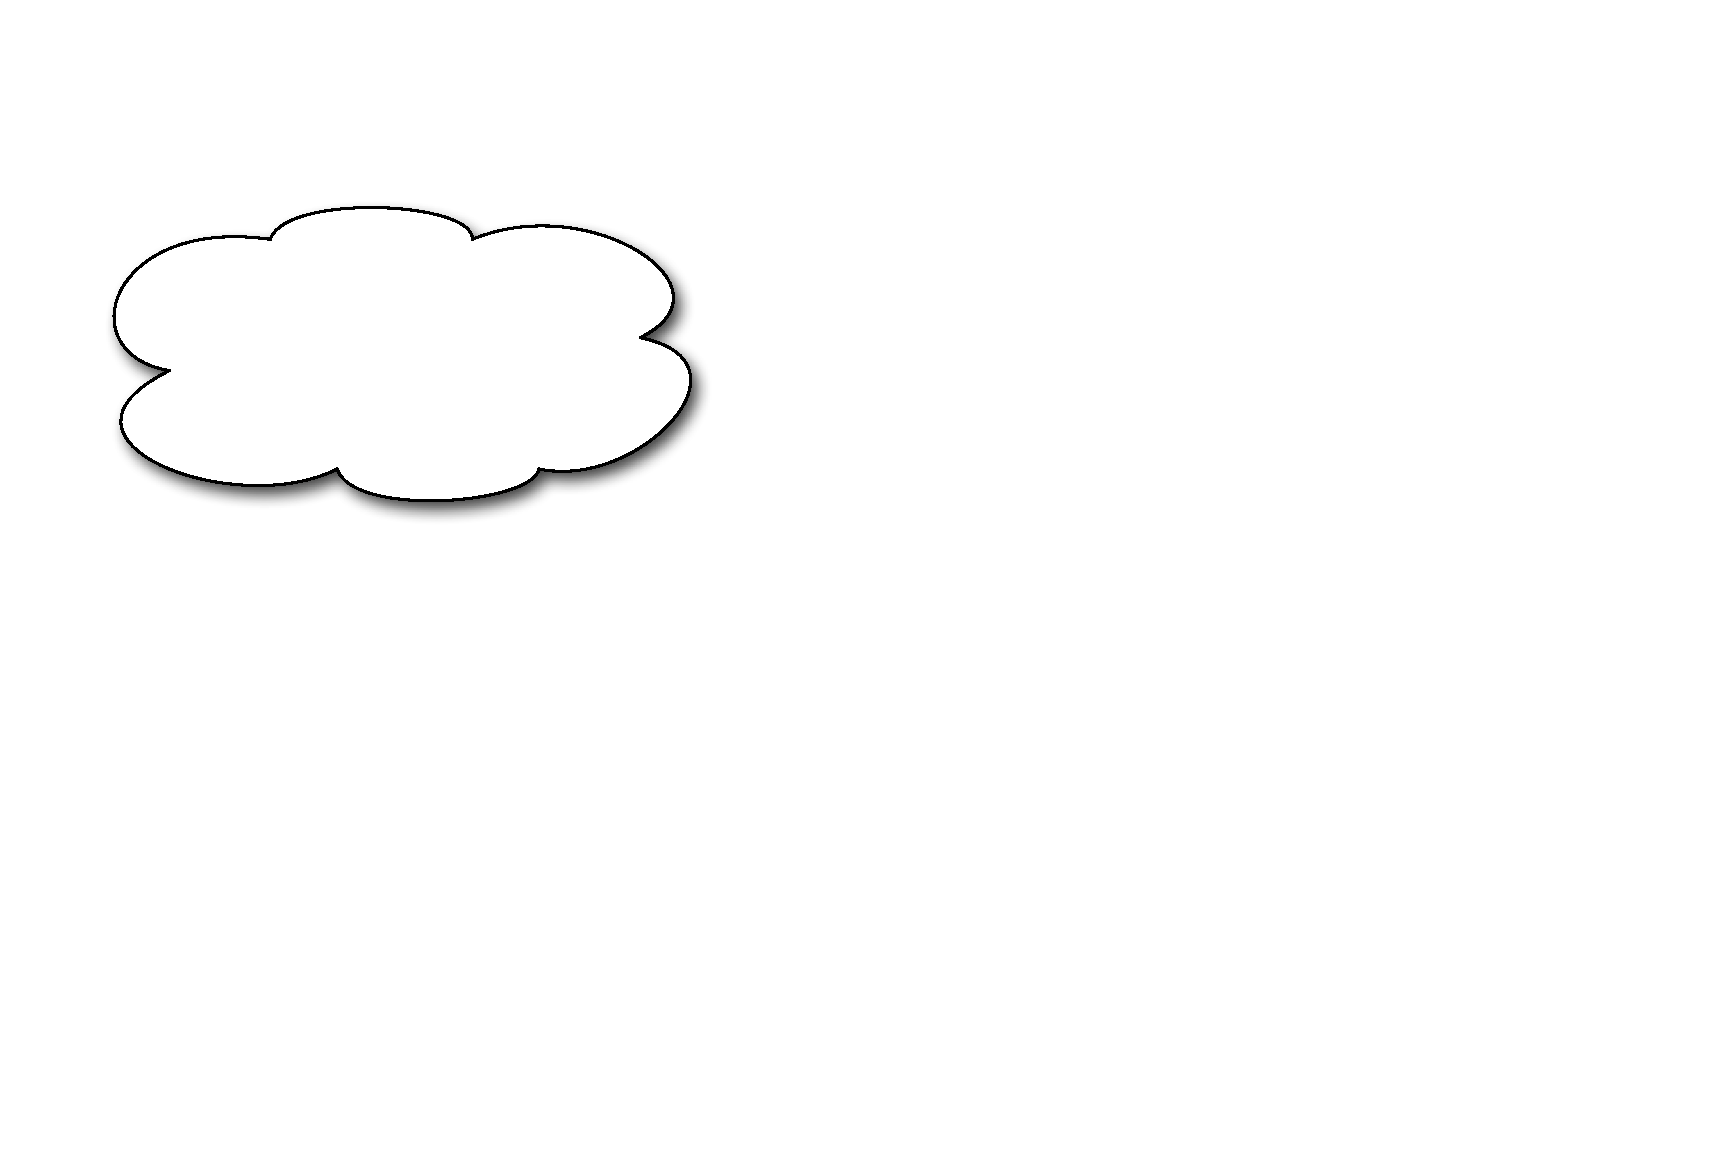
\includegraphics[scale=.4]{figure-stacking.eps}
\caption{Stacking PCB construction}
\label{fig:stacking}
\end{figure}

Secondly, dividing the board into two allows the ``main'' board to be
designed with production use in mind, without any restrictions from
Arduino compatibility.  The second board provides Arduino
compatibility and other development facilities.  Consequently, we denote
the lower ``main'' board as the {\it production} board and call the
upper, Arduino-compatible board as the {\it development} board.

In the new design, the production board essentially hosts all the
components in the current prototyping board in a smaller form factor.
However, instead of having the Arduino-compatible 100 mil female
headers, it has a pair of low-profile board-to-board connectors,
providing connectivity with the development board or any other
extension board.  Furthermore, the production board is designed in a
fashion that allows it to be devided into two parts, one part hosting
the MCU, the Ethernet chip, and the I/O subsystem, the other part hosting the
PoE signalling, DC/DC PSU, and Ethernet magnetics.  When separated,
these two boards may be connected with seven wires, allows them to be
placed inside the device in a flexible manner.  This is illustreated
in Figure~\ref{fig:divided}.

\begin{figure}
\centering
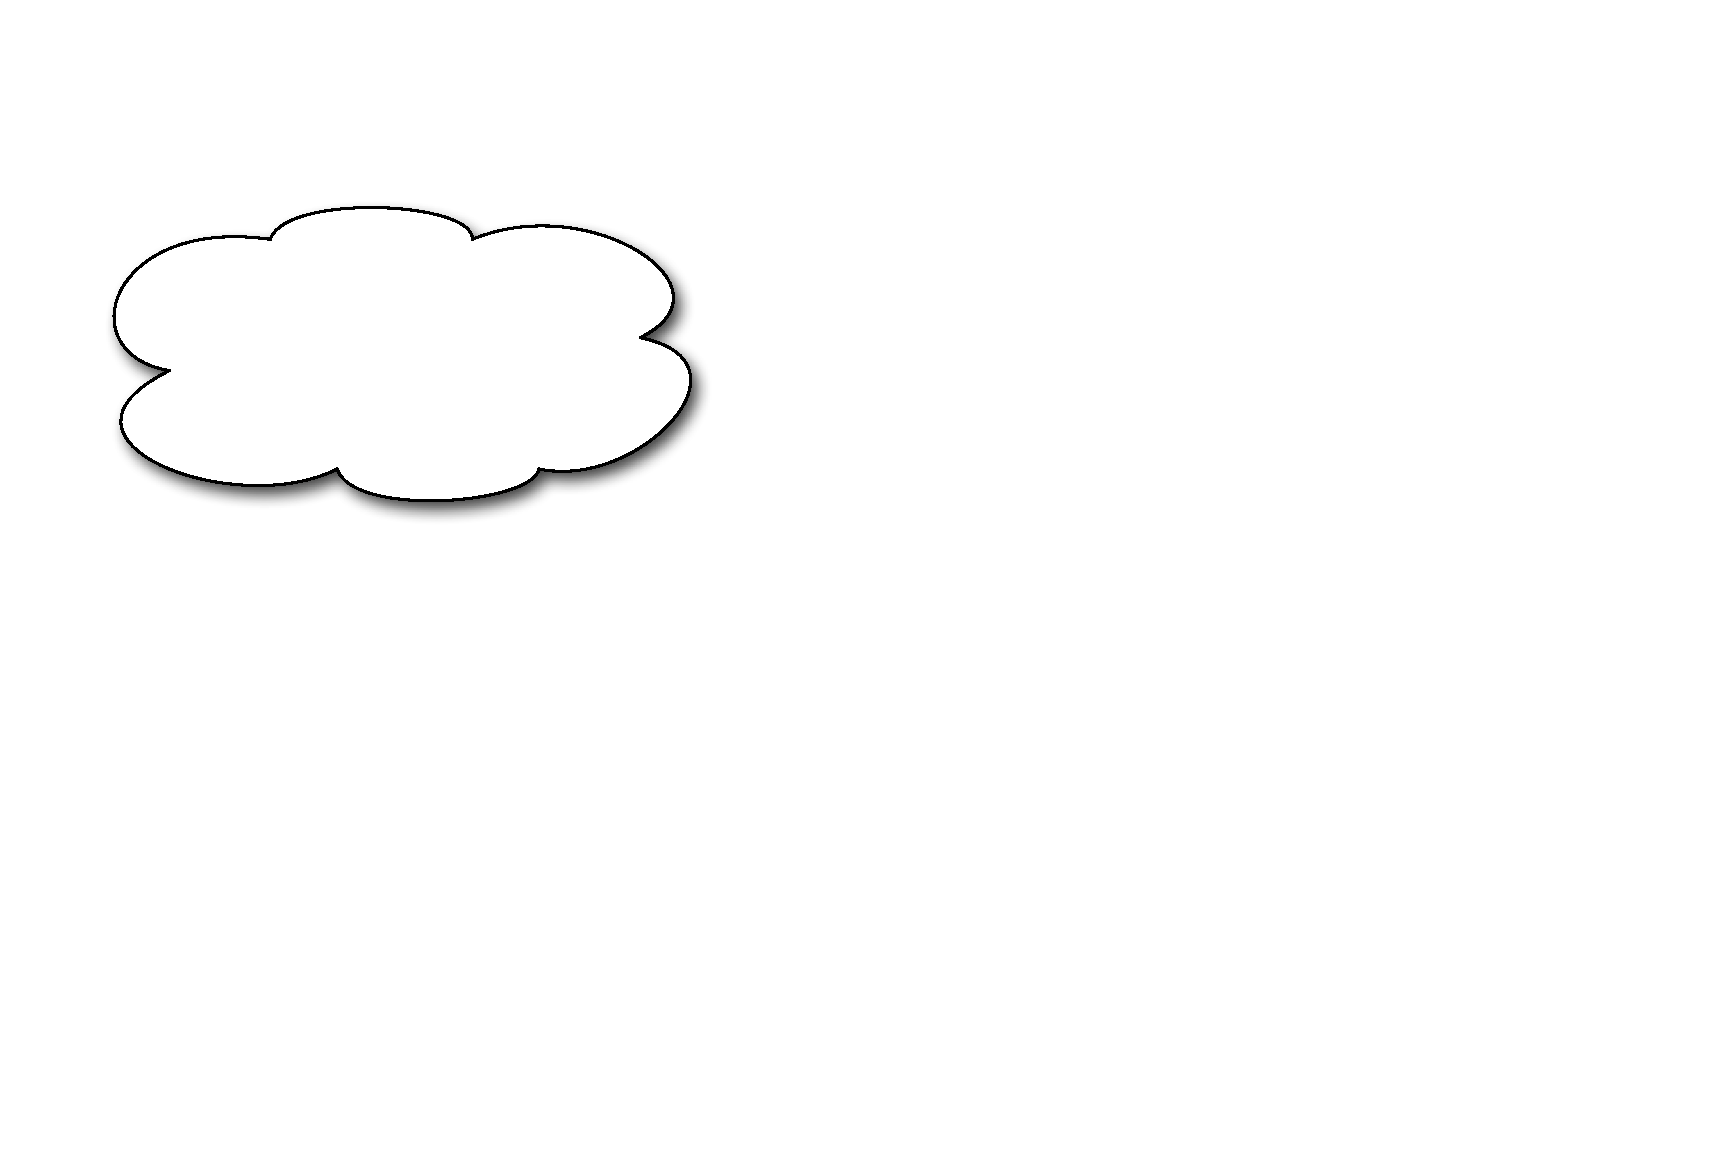
\includegraphics[scale=.4]{figure-divided.eps}
\caption{Two-part PCB}
\label{fig:stacking}
\end{figure}

The development board, in turn, hosts the Arduino-compatible headers,
and USB slave chip that can be used for flashing and debugging the MCU
on the production board, and a number of low-current LEDs which may be
used to monitor the I/O state at the Arduino-compatible connectors, and ability
to provide 5V power from the USB connector, thereby allowing the board
to be used even when powered only via the USB connector.

{\bf Other hardware enhancements.}
According to the datasheet, the flyback controller on the LTC4267 chip
is capable of using any input voltage between roughly 11 and 60
volts\footnote{Care must be taken in generating the initial
boot-time operating voltage for the LTC4267 chip so that it is placed
at the right range of roughly 7--9V.}.  Hence, in the next revision we
attempt to allow the board to be powered at any voltage in the range
of 11--60V, both through the external power connector and over the
spare pairs on the CAT5 cable.  The selection between PoE-compatible
powering and other powering will take place with a jumper.  When
alternative powering is used, care must be taken not to draw too much
power as the PoE-built-in current limitation will not be in use.

One of the benefits of using the STM32F series MCUs is that they have
been designed to be (almost) pin compatible in various packages.
Hence, in the 64-pin packages that we are using we can design the PCB
to host MCUs ranging from the low-end STM32F050 Cortex-M0 one to the
high end STM32F407 Cortex-M4 one, with just a few simple solder
jumpers.

While we are not planning to add any additional placed components on
the production board, in order to keep it at a low cost, we plan to
add unplaced pads for supporting an RTC, operational amplifiers, level
shifters, and driver FETs which may be used when connecting the MCU
I/O pins various sensors and power devices.  The production board is
planned to include 100 mil spaced soldering holes on both of its long
sides, for directly connecting external devices or for adding male
headers to plug in the production board to a breadboard,

On the mechanical side, the plan is to allow one to use
punch-down Ethernet connectors~\cite{Krone} instead of the RJ45 jack
for fixed installation.  The metal case is planned to host the
production board together with any extension boards of the same
dimensions.

\subsubsection{Software efforts taking place}

At the moment we are extending the existing Arduino-compatible runtime
with a simple pre-emptive scheduling system, thereby allowing the uIP
TCP/IP stack to run in parallel with any Arduino sketch.  We are
considering whether we should support a more full fledged real time
operating system (RTOS), such as ChibiOS/RT~\cite{ChibiOS}; at this
writing the question is still open.

Once we will have basic TCP/IP up and running, the next step is to
start integrating the system with cloud components.  The exact plan
for this is still open.  Finally, proper cloud connectivity will
enable secure remote software updates.

\subsection{Design choices}

% XXX This section needs more work, or needs to be removed

With the ELL-i platform, our goal has been to produce an easy-to-use,
flexible, and inexpensive platform for fixed appliances.  These goals
have guided our design choices.  Indeed, the primary choice of using
Power-over-Ethernet stems from this goal, as it allows us to use a
single cable for both power and communications, thereby potentially
reducing the overall cost while still being flexible and easy-to-use.

Considering the component choices in the first prototyping board, we
have tried to select the lowest-cost components that are easy-to-use
and flexible enough.  Consequently, we opted for the lowest end ARM
series, Cortex-M0, as they are easy-to-use as a familiar 32-bit
platform and most likely to hit the lowest price point in the area
within a few years\footnote{At the moment, there are still older
  Cortex-M3 based MCUs on the market that are sold cheaper than the
  newer Cortex-M0 MCUs in small lots.  However, the lowest price
  point is most likely to be replaced with the Cortex-M0 MCUs within
  the next couple of years.}.
The chosen Ethernet chip is the lowest-cost denominator of those
widely used in the market.  At the PoE and DC/DC PSU side there is
still room for optimisation, but we are currently planning to leave
that for later.

For hardware-level expandability, we are still working to determine
the right approach.  At the moment, we are using the Arduino-compatible I/O
connector design for development-time extensions.  However, it is
clear that they are not a good choice for production use, for many
reasons\footnote{The Arduino-compatible connectors are physically quite large,
  requirign more space than what is available within many devices and
  e.g. within a pattressbox.  Furthermore, the Arduino-compatible connectors are
  basically unbuffered, making it somewhat tricky to get good ADC
  readings or driving higher loads through them.}.

Considering the connectors and mechanics, our goals are again the
same: easy-to-use, flexible, and inexpensive.  For Ethernet, the goal
is to support both the familiar RJ45 connectors and the punch-down
connectors for fixed design, the punch-down connectors being clearly
cheaper.  In the new design, we are looking at various options for the
connectors between the production and development boards.  At the
moment, we are planning to allow different approaches for tying the
boards together, including using screws and having suitable notches in
the packages.

At the firmware side, it looks likely that we will end up implementing
our own runtime.  Looking at the various open source RTOS options
available, they typically include more than what we need and with a
license that is not fully compatible with our planned business model;
see below.  The cloud-side components will be based on the lowest
common platform-as-a-service (PAAS) denominator, which at the moment
seems to be the Amazon Web Services (AWS)~\cite{AWS} APIs, also supported by
e.g. the AppScale~\cite{AppScale} open source framework.

% ------------------------------------------------------------------

\section{Application examples}
\label{sec:examples}

As a platform, the ELL-i design is open ended.  In this section, we
briefly describe a few designs that we presume the ELL-i platform
making easier or less costly to implement than before.  Furthermore,
wherever applicable, we attempt to illustrate how the open source
nature of ELL-i will benefit the individual applications.

\subsection{Illumination}

The very first demo that we implemented using ELL-i, while the
platform was still a set of evaluation kits bolted to a wooden board
and wired together, was a driver for a commercial high-power RGB LED
projector.  Since then, we have repeated the LED driver exercise a few
times.

From the electronics point of view, an adjustable HP LED driver is a
relatively simple device, as LEDs in general are current-driven
components.  That is, the voltage drop over a LED remains relatively
constant independent of how much current is flowing through the LED,
and the amount of current determines how brightly the LED shines.  The
typical voltage drop over a HP LED is around 3V.  Hence, for driving a
LED from a voltage source that is higher than the voltage drop of the
LED it is enough to limit the amount of current.  For indicator LEDs
the current is usually limited with a suitable series resistor;
however, such an arrangment would be very inefficient for driving an
HP LED out of the PoE nominal 48V.  Fortunately, a buck
converter~\cite{buck-converter}, the simplest of the so-called
switching mode power supply (SMPS)~\cite{SMPS} topologies, is quite
easy to regulate to produce a constant, adjustable current.  All that
is needed is a simple current-measurement circuit and a simple
algorithm to drive the switching FET in within the driver.  While
achieving high efficiency requires somewhat more work, even an
electronics amateur, like us, is able to design a simple
MCU-controlled buck converter in a couple of weeks time.

So, it looks like that from the hardware point of view, driving
LED-based lamps would be an ideal application for the ELL-i platform.
In addition to the components already in ELL-i, a LED driver at its
simplest format requires a switching FET, a choke coil, a diode for
the sustained current from the coil when the FET is not conducting,
and a current measurement circuit consisting of a shunt resistor and
an operational amplifier.  In a practical design, a few more
components are needed, but their additional cost is a few cents.

Consequently, ELL-i may be an excellent platform for implementing
future, more intelligent show lighting systems, flexible retail
lighting, and other illumination applications where it is beneficial
to control each and every lamp separately.  In such an environment,
ELL-i implements the yesterday maxim of each light bulb having its own
IP address~\cite{lightbulb}.

To communicate with the external world, and ELL-i node may implement
the Ethernet or TCP/IP variants of the commonly used lighting control
protocols, including DALI\cite{DALI} and DMX\cite{DMX}.

\subsection{Automation}

Another area where the ELL-i platform may bring benefits is building
and industrial automation.  In the building automation area, there are
already a number of Power-over-Ethernet products at the market,
including locks and other security and safety equipment.  However, to
a large extent the existing automation systems are still based on
standards, such as KNX\cite{KNX}, BACnet\cite{BACnet}, or
LonTalk\cite{LonTalk}, which generally utilise twisted pair
control cables with separate power supply.

From that point of view, ELL-i provides an open source platform to
build upon.  As such, ELL-i provides little benefit directly to
automation, as it is lacking direct connectivity with sensors and
actuators, and it does not as such implement any of the existing
protocols.  Therefore, as a standalone component it does not integrate
with the existing automation systems.

However, ELL-i is a small, connected, intelligent, power-convoying low-cost
component, the ELL-i platform provides a platform.  Therefore it could
potentially be co-located with the sensors and actuators, providing
power to them and integrating both intelligence and connectivity
directly to them.  Consequently, it would allow replacing the
hierarchy of separate field devices (sensors and actuators) and the
programmable logic controllers (PLC) with a flat logical hierarchy,
allowing the physical connectivity to be arranged in any topology.

Beyond the basic functionality challenges, applying ELL-i in
automation systems would require a number of non-functional challenges
to be addressed.  First and foremost, it should be demonstrated that
the ELL-i system is reliable as the known and proven old solutions.
As it is unlikely to happen as such any soon, one way to address the
reliability concern is to build reliability through redundancy.  That
is, a system consisting of the ELL-i platform based nodes can be
engineered to be inherently redundant, placing two ELL-i nodes at each
sensor or actuator side, using standard Ethernet network redundancy
approaches\footnote{Dual cabling with redundant switches, spanning
  tree protocols to avoid bridging loops, etc.}, and addressing
software-level redundancy through differing runtime systems.

\subsection{Education}

A third area where ELL-i may turn out to be useful is education.  As
an open system, ELL-i itself can be studied and modified by the
students.  Secondly, as an easy-to-use embedded system ELL-i may be
used in various student projects where real-life interaction is
needed.  We already have some experience on this; see below.  Finally,
the ELL-i system itself may be extended to be a platform for teaching
basic programming in a fun and easy-to-understand way.

\subsubsection{ELL-i platform itself as course material}

The ELL-i platform has been designed to be not only easy to use but
also easy to understand.  The hardware represents a complete design
with an MCU, Ethernet-based communications, and a DC/DC PSU.  The
chosen MCU is a relatively simple but still powerful one, from a
family that is commonly used in open source projects.  The CPU core
within the MCU is a modern 32-bit RISC architecture with simple
3-stage pipelining and no instruction reordering, being easy to teach
and to understand.  The MCU-related prt of schematic is very similar
to the relevant part of the MCU manufacturer's evaluation board.  The
Ethernet communications module consists of a single chip and the
magnetics and has a wide support in the open source community.
Finally, the DC/DC PSU is a relatively simple buck converter design
that can be understood in a few days with a basic analogue electronics
background.

At the software side, the firmware has been written in a modular
manner, as was explained above in Section~\ref{sssec:runtime}.  Hence,
studying simple firmware designs that do little but initialise the MCU
and blink some LEDs is relatively easy.  The modularity then allows
more complex features, such as communications and scheduling, to be
added in a piecewise manner to the design.  This allows the teacher to
demonstrate the full runtime in a gradual manner, starting from MCU
initialisation and simple I/O, continuing through the SPI and I2C
protocols up to simple Web services.

Hence, the ELL-i platform may be used to introduce and demonstrate all
the elements of a modern Web-connected computer, including both the
hardware and software, without the complexities present in the typical
moder computers.

\subsubsection{ELL-i as a student project platform}

Due to the simplicity and the modular design of the ELL-i platform, it
is a relatively easy platform for students to build their platforms
upon.  Arduino compatibility allows adoptation of almost any of the
some 300 existing Arduino shields, typically with some minor
software-side modifications.  In many cases, the more powerful MCU on
the ELL-i platform allows the sensors or other components on the
shield to be used more intelligently than with the basic Arduino
boards.  Ethernet-based powering allows the devices to be placed
relatively freely anywhere, thereby allowing the students to build
smart spaces or place smart fixed devices at desired locations.

The simplicity and flexibility of the platform also allows the
students to replace many parts of the platform with their own
components.  For example, at this writing, a student group at
University of Turku have completed a preliminary port of the
FreeRTOS~\cite{FreeRTOS}.

{\bf EIT Smart Spaces summer school.}
In June 2013, a couple of weeks after the first ELL-i prototyping
boards had arrived, two of us held a one-day ELL-i tutorial at the
European Institute of Innovation and Technology (EIT) Smart Spaces
summer school in Grenoble, France.  The tutorial lasted for six hours,
within which the computer science students built a simple buck
converter based LED driver, using the ELL-i platform, discrete
components, and the Arduino IDE.

During the tutorial, the students learned how to handle basic physical
electronic components, including resistors, capacitors, coils, FET
transistors, diodes, and LEDs.  Starting from a very simple design,
they built in a stepwise manner an adjustable constant-current DC/DC
converter that generated some 300 mA of current from the nominally 48V
unregulated DC power available from the PoE header on the ELL-i
prototyping board.  The background of the students varied from ones
that had only taken theoretical basic courses in electronics, as a
part of their basic studies, to a few that had built simple
Arduino-based prototypes before.  None of the students had any idea of
how the DC/DC power supplies actually work.


\subsubsection{ELL-i as an educational tool}

With relatively simple extensions, ELL-i has potential of becoming a
platform for teaching the basics of programming.  With today's
computers and smart phones with fancy graphical user interfaces,
writing very basic programs that only print on a console log is
unexciting.  On the other hand, with an Arduino-like platform even a
simple program can light up LEDs and affect real-life things.  With
its powering capability ELL-i adds there the ability of doing ``real''
things as such, such as driving solenoids or even motors.

Given that the Arduino APIs and sketches are C++ programs in practise,
it would be possible to write a set of C++ proxy classes and templates that
compile an Arduino sketch so that it runs in an emulator, allowing the
functioning of such a sketch to be simulated and illustrated on a PC.
Furthermore, with the Ethernet interface, another set of proxy classes
could be used to instrument a sketch, allowing it to be run on the
ELL-i platform while simultaneously inspecting the variables and I/O
ports.  In practise the instrumentation classes would communicate the
application state over the Ethernet to a PC, which would then use the
simulator user interface to illustrate the application state.
 
% ------------------------------------------------------------------

\section{Business model}
\label{sec:business}

In this section, we briefly look at the ELL-i business model, which
somewhat deviates from most typical business models, being closer to
to the Linux kernel community~\cite{Linux-kernel-need-reference}
and XXX~\cite{Something-else-need-reference}.

As stated, the goal of the ELL-i project include providing an
inexpensive and easy-to-use platform for all kinds of fixed
appliancies.  As always, in electronics production achieving a low
price requires high volumes.  Hence, the ELL-i business model aims to
make the platform widely available at a low cost, thereby encouraging
it to be widely used, leading to increasing volumes and thereby even
lower prices.  In other words, the project does not aim to
create profits as such but to distribute the added value in the form
of lower prices, thereby contributing to the economy as a whole.

The ELL-i project itself has been incorproated as a co-operative, with
the intention that the hardware and software copyrights are co-owned
by the developers.  That is, the aim is that the co-operative owns the
copyright for all of the hardware and software components within the
core ELL-i platform and the developers who contribute to the project
may join the co-operative as members if they wish to do so.

We envision that the project and the co-op will create interest among
commercial for-profit companies.  This is important both for creating
volumes and for distributing the created value to the economy.
Hence, the ownership, governance and licencing models have been
planned and will be adjusted to make the platform lucrative for
commercial licensees.

However, in order to get the platform there in the first place, we
first need to entice a group of enthusiastic developers that want to
contribute to the project.  For that, we presume that we first need to
sell a few thousand boards.  Based on studies in similar kinds of
situations~\cite{need-reference}, we expect that 1--4\% of the early
% XXX Check the percentage above
adopters will turn into active developers; see
Section~\ref{ssec:earlymarket} below.

Hence, the ELL-i business model needs to be balanced between the early
market need of creating a sizeable developer community and the
somewhat later need of attarcing commercial companies in order to
create volumes and benefitting the larger society.  We attempt to the
address these somewhat conflicting needs through separating the
ownership, governance and licencing practises; see
Sections~\ref{ssec:ownership} and~\ref{ssec:licencing} below.

The resulting structure has probably a relatively low monetary value
compared to its overall utility value, as the ownership will be more
anchored than in most alternative models.  However, we consider this
as a virtual from the macroeconomic
perspective~\cite{Olson2002}, somewhat similar to what
state-owned enterprises provide but deteched from the populistic
political system.

\subsection{Early market challenges}
\label{ssec:earlymarket}

At the moment, the main challenge ELL-i faces is a marketing one.  The
first version of the hardware platform exists both as open source
schematics and layout and as actual, functioning hardware boards.  The
software platform is being continuously enhanced, providing the basic
facilities that are needed to get started.  However, the group of
active developers is quite small, just a handful of people working
mostly on their spare time.  In order to get the ball rolling, more
active developers are needed.

We believe that the ELL-i approach of providing both power and
communications over a single cable is beneficial to a fair number of
people, especially when the incoming power can be easily converted
into a DC voltage suitable for various kinds of loads.  Hence, from
the ELL-i point of view, a major challenge is to find the people that
are already struggling with the appliance powering problem and
demonstrate the viability of the ELL-i solution.  That in turn
requires both much more visibility than what ELL-i enjoys today and a
number of additional power supply designs, making it easier to have
suitable power tailored for each load.

An initial market presense may be achieved through crowdsourcing,
e.g. through a Kickstarter~\cite{Kickstarter} campaign.  That may help
with gaining initial production volume and inducing a few new
developers; however, such a campaign is also likely to saturate the
early market, making it considerably harder to sell new hardware for a
while.  Hence, at the time a crowdsourcing campaign is commenced,
there must be sufficient structure in place so that the new developers
have a clearly laid approach and incentive to start contributing to
the project.

What comes to the powering of appliances, we basically need to learn
ourselves -- within the core group -- to build a more diverse set of
power supplies.  We also need to make the resulting knowledge
available in an form that is easier for relative newcomers to apply
than the currently available information, initially as recipies and
later on as ready-applicable DC/DC converter units.  The basic ELL-i
recipe for providing adjustable constant-current power is already
there, thereby enabling adjustable LED drivers, and we expect to
complete our first design for inductive loads, such as solenoids and
motors.

%\subsection{Ownership and governance models}
%\label{ssec:ownership}
%
%ELL-i open source co-operative was founded in June and the first
%bylaws were officially accepted only in this September.  In this first
%set of bylaws a considerable amount of power is given to the co-op
%board, trusting the initial board to have the right incentives in
%establishing suitable ordinances for future governance.  At the same
%time, the official ownership model is completely flat and egalitarian
%in the original spirit of co-operatives, treating all members equal.
%Each member may only have one membership share.
%
%The current bylaws state that the board accepts new members.  Each new
%member shall have a single membership share and they are oblidged to
%pay the membership fee and a sign-up fee.
%
%The mutual understanding within the current membership is that the
%board will only accept people and businesses who have contributed to
%the project.  In this early stage, though, the board may also accept
%members that only have a plausible intention to contribute instead of
%having already contributed.  The board may also adjust the sign-up fee
%downward; e.g., in the case of members joining from developing
%countries.   On the other hand, new members may opt to purchase
%supplementary shares to support the co-operative.
%
%While the ownership model is egalitarian, the governance model is
%meritocratic.  That is, it aims to give more power to those members
%that have contributed and are contribution most to the co-operative,
%while less-contributing members have less power.  At the moment, the
%bylaws state that the board divides the members into three groups
%based on their contributions to the co-operative.  Those having
%contributed most have 10 votes in the co-operative assembly, those in
%the medium category have 3 votes, and the remaining members just one
%vote.  This model is presumed to suffice in the beginning.
%
%As the co-operative grows and the members no longer know each other at
%the personal level, we expect that the governance model and maybe also
%the ownership model will need revisions.  However, as there is no way
%to know what model might serve the co-operative best, we assume that
%the co-operative needs some organisational innovation and
%experimentation.  The current presupposition is that once the number
%of members passes Dunbar's number~\cite{reference-needed}, such
%experimentation will become harder and more of the governance needs to
%be formalised into the bylaws.
%
%\subsection{Licencing model}
%\label{ssec:licencing}
%
%While the ownership and governance models are important for the
%developers and the evolution of the co-operative structure, the
%licencing model is expected to be a cornerstone of the success of the
%platform.  At the moment, the exact way how the platform will be
%licenced is still in the works.  It looks like that it will be
%licensed with simultaneously with three different licenses, one aimed
%for hobbyists, one for commercial companies that want to use the
%platform in their products but that are not interested in contributing
%back, and one for commercial companies that want to be part of the
%community.  In the following two subsections we consider the case
%first from the developers' point of view, and then from the commercial
%licencees' point of view.
%
%\subsubsection{Developer incentive structure}
%
%The developers are the main ``raw material'' for any open source
%initiative.  Our goal is to make it easy to become a developer and
%encourage the developers to continue staying community members,
%building a sustainable group of ``core'' developers.
%
%In principle, the set of potential incentives for
%engaging developers are extrinsic motivators, such traditional
%currencies (money) and money-like alternative
%currencies~\cite{Liataer2001}, and intrinsic and internalised
%extrinsic incentives, such as fun, reputation, learning, and personal
%use~\cite{von2012carrots}.  The internalised extrinsic incentives
%include social aspects such as community respect and membership in an
%exclusive community.
%
%According to conceptual process modelf of sustained participation, as
%introduced by Fang and Neufeld~\cite{fang2009understanding}, an open
%source project needs a large pool of potential candidate developers in
%order to build a sustainable base of core developers.  To attrack such
%candiates, the project needs to be easily accessible and the platform
%needs to be useful, creating an initial motivation based on expected
%personal use.  The ELL-i platform aims to reach these goals through
%making the platform easy to use, marketing the platform widely in the
%open source community, and producing a number of example designs that
%are useful as such.
%
%Once a project has a large-enough pool of candidate developers, the
%project should support a continuous participation cycle that fosters
%situated learning and identity construction.  That is, there should be
%a clear learning path for new developers so that they may easily start
%contributing to the project through conceptual suggestions and
%practical doing, allowing them to establish a known ``name'' (communal
%respect) within the community~\cite{fang2009understanding}.
%
%We postulate that such sustained participation created initially
%through personal utility and later mainly through communal respect and other
%social factors may be further strengthened via non-convential
%extrinsic factors, resembling Lieataer's alternative
%currencies~\cite{Lietaer2001}.  Examples of such incentive mechanisms
%may be both non-transferable or even convertible ``contribution tokens'',
%denoting a developers' overall level of contribution to the project
%over time or allowing them to financially benefit from their
%contributions.
%
%At the present, the idea is that a typical developer ``career'' would
%consists of the following steps:
%\begin{enumerate}
%  \item Anyone may become a (private) developer through downloading
%    the source code and making their own modifications.
%  \item Those developers that want to contribute their modifications
%    to the core, for example due to extrinsic or intrinsic factors,
%    must donate the copyrights to the co-operative.
%  \item The co-operative may accept such copyright donations or not,
%    thereby creating a gradually tightening quality control barrier.
%  \item The developers whose copyright donations have been accepted to
%    the core may formally join to the co-operative as full members.
%  \item The full members of the co-operative govern the co-operative
%    an get extrinsic membership benefits, such as discounts on future
%    versions of the hardware or special non-money or alternative-mony
%    tokens denoting the significance of their contributions.
%\end{enumerate}
%
%\subsubsection{Commercial licensee incentive structure}
%
%Let us now look at the situation from a commercial licensee point of
%view.  When considering the ELL-i platfrom, a company has a number of
%choices: they may decide to use the ELL-i platform using the open
%source license, they may decide to license the ELL-i platform under a
%different license, they may decide to use another platform, or they
%may decide to build their product without any external platform at
%all.  Each of these choices have their pros and cons, whose closer
%analysis falls beyond the scope of this paper; here we merely list a
%number of preconditions without which the choice of licensing ELL-i
%under a commercial license will not be attractive at all.
%
%For a commercial license to be more attractive than an open source
%license, the open source license needs to be somehow more restrictive;
%for example, if the open source license is a GPL variant, the
%``virality'' of the GPL may be considered as a drawback.  For ELL-i to
%be more attractive than some other platform or in-house development,
%it shall provide tanglible benefits, such faster time-to-market,
%lower investment costs, lower maintenance costs, or higher quality.
%
%In addition to the initiali licensing decision, we also need to
%consider the incentives for a commercial company to contribute back to
%the community in the form of donated code or other technology.
%In addition to the ownership and governance benefits stemming from
%membership, companies may also benefit form of network effects
%stemming from platform standards
%(cf.~eg.~\cite{gandal2002compatibility}) and the ability to influence
%them.
%
%While we have a relatively good understanding how the incentive model
%might work for individual developers, our understanding of the detals
%of the licensing model are still in the works.
%
%\subsection{Business model summary}
%
%As a first approximation from the conventional economics point of
%view, the ELL-i platform seems to form a fairly classical two-sided
%market~\cite{rochet2003platform}.  ELL-i offers the platform
%essentially free-of-charge to the developer community, allowing
%individual developers to innovate and fulfil their personal needs.  At
%the same time, it offers the platform for commercial companies for a
%fee.  However, at the same time it attempts to form a joint community
%of both individual developers and products companies, creating a
%larger two-sided market where the sides are the hardware component
%manufacturers and the product users.  From that point of view, ELL-i
%benefits the component suppliers through larger volumes, the product
%companies through increased bargaining power, and the product users
%through increased variety and lower average price of the products.  A
%more detailed analysis of the market structure is in the works.
%
%From a societal point of view, if ELL-i succeeds as a platform it may
%produce essentially a virtual non-profit monopoly, benefitting the
%society through the increased efficiency of scale of the used
%components and overall lower user prices of the technology.  At the
%same time, its egalitarian ownership structure anchors the forming
%intellectual capital within the community while the meritocratic
%governance structure allows any further development to be primarily
%technology driven, aiming for long-term engineering excellence instead
%of short-term profits.

% ------------------------------------------------------------------

\section{Ongoing work}
\label{sec:ongoing}

As a platform and a business model, ELL-i is still at its infancy.  As
a development platform, we are still busy laying out the building
blocks: the next version of the hardware is being worked on, the
software is receiving constant inprovements, and at the tools side we
are smoothing out the developer path from the easy-to-start-with but
simplistic Arduino IDE to the more powerful full-fledged tools.  At
the same time we are looking at how to expand the technology to conver
a wider variety of environments; for example, it would be very
desirable to use the ELL-i platform without requiring any new cabling
when renovating existing installations.

From the community building point of view, ELL-i has but started yet.
We are still considering how to best launch a campaign to expand the
developer base beyond the founders of the co-operative.  It seems
clear that we need some sort of a crowdsourcing campaign to attract
developers and to gain initial volumes.

Finally, the governance and licencing models clearly need much more
work.  Our understanding of how to structure the business model in a
way that allows both fast organic growth and sustained technical
development is still inadequate, requiring both better theoretical
understanding of the various stekeholder incentives and real-life
experimentation in the form of trying out a few alternatives.

% ------------------------------------------------------------------

\section{Conclusions}
\label{sec:conclusions}

Realising the Internet-of-Things (IoT) and Machine-to-Machine (M2M)
visions will make our environment immensely contextual in the sense
that the digitally interconnected artifacts in our environment may
jointly form a rich model of what is taking place in any given space,
allowing the environment to react in a smart manner.  In this paper,
we have discussed one potential step towards that vision, the ELL-i
initiative and technical platform.

The ELL-i initiative is organised as a co-operative, with the
intention of producing inexpensive open source hardware and software
for wired appliances and implements, such as aquariums, bowling
alleys, cooktops, dishwashers, the way to toasters, underlayments,
vacuum cleaners, washers, xerox machines, yachts, and kitchen zinks.
The currently available ELL-i prototyping board allows researchers and
other developers to explore the ELL-i approach, creating prototypes of
intelligent, communicating things that can be readily located anywhere
at the distance of an Ethernet cable.  With its Arduino compatibility,
the ELL-i platform provides a very low entry barrier, while still
outlining a clear path for more powerful approaches.

From the technical point of view, the main promise of the ELL-i
approach is in its ability to provide reasonable amounts of electrical
power, combined with the communication and data processing capability,
at a very reasonable price point.  If ELL-i ever reaches
mass-production quantities, it will provide an electronics module that
allows almost any wired electrical device to be converted into its
``smart'' equivalent at the additional production cost of just a
couple euros.  Consequently, as even a typical light switch or toaster
is priced at a level close to or exceeding ten euros, that may
gradually enable complete ``smartification'' of our urban
environment. 

The ownership, governance, and incentive models built into the ELL-i
co-operative have been designed with sustainability in mind.  They aim
to create an openly governed, jointly owned platform that is firmly
anchored within the society and developed as an essentially public good.

\section*{Acknowledgments}

The authors would like to TBD.

\bibliography{scpe2013}{}
\bibliographystyle{plain}

\end{document} 

